\section{Inverse Functions}\label{sec:inv_funcs}

We say that two functions $f$ and $g$ are \emph{inverses} if $g(f(x))=x$ for all $x$ in the domain of $f$ and $f(g(x))=x$ for all $x$ in the domain of $g$. A function can only have an inverse if it is one-to-one, i.e. if we never have $f(x_1)=f(x_2)$ for different elements $x_1$ and $x_2$ of the domain. This is equivalent to saying that the graph of the function passes the horizontal line test. Functions that are not one-to-one may sometimes have inverses on part of their domains.

If $f$ and $g$ are inverses, the domain of $g$ will be the range of $f$ and the range of $g$ will be the domain of $f$. The graphs of $f$ and $g$ will be reflections of each other across the line $y=x$ since $y=f(x)$ if and only if $x=g(y)$ (since the point $(y,x)$ is on the graph of $g$ whenever $(x,y)$ is on the graph of $f$.)  The inverse of $f$ is denoted $f^{-1}$, which should not be confused with the function $1/f(x)$.

To determine whether or not $f$ and $g$ are inverses for each other, we check to see whether or not $g(f(x))=x$ for all $x$ in the domain of $f$,and $f(g(x))=x$ for all $x$ in the domain of $g$.

\youtubeVideo{BmjbDINGZGg}{Finding the Inverse of a Function or Showing One Does not Exist, Ex 3}

\example{ex_inv_determine}{Verifying Inverses}{Determine whether or not the following pairs of functions are inverses:
\begin{itemize}
\item[(a)] $f(x)=3x+1$; $\displaystyle g(x)=\frac{x-1}3$
\item [(b)]$f(x)=x^3+1$; $g(x)=x^{1/3}-1$
\end{itemize}}{\begin{itemize}
\item [(a)] To check the composition we plug $f(x)$ in for $x$ in the definition of $g$ as follows: \[ g(f(x))=\frac{f(x)-1}3=\frac{(3x+1)-1}3=\frac{3x}3=x\]
So $g(f(x))=x$ for all $x$ in the domain of $f$. Likewise, you can check that $f(g(x))=x$ for all $x$ in the domain of $g$, so $f$ and $g$ are inverses.
\item [(b)] If we try to proceed as before, we find that:
\[ g(f(x))=(f(x))^{1/3}-1 =(x^3+1)^{1/3}-1\]
This doesn't seem to be the same as the identity function $x$. To verify this, we find a number $a$ in the domain of $f$ and show that $g(f(a))\neq a$ for that value. Let's try $x=1$. Since $f(1)=1^3+1=2$, we find that $g(f(1))=g(2)=2^{1/3}-1\approx 0.26$. Since $g(f(1))\neq 1$, these functions are not inverses.\eoehere
\end{itemize}}

To find the inverse $f^{-1}$ of a given function $y=f(x)$, we follow these steps (when possible):
\begin{enumerate}
\item In the equation defining $f$, solve for $x$.
\item Interchange $x$ and $y$.
\item The equation now defines $y=f^{-1}(x)$.
\end{enumerate}

\example{ex_inv_find}{Finding Inverses}{Find the inverses of the following functions.
\[\text{1. }f(x)=5x+3\qquad\text{2. }g(x)=x^3+1.\]}{\begin{enumerate}
\item Start with the equation $y=5x+3$ and solve for $x$:
\begin{align*}
y&=5x+3\\
y-3&=5x\\
\frac{y-3}5 &=x
\end{align*}
Next interchange $x$ and $y$ to get $y=\dfrac{x-3}5$. The inverse of $f$ is:
\[ f^{-1}(x)=\frac{x-3}5 \]
\item Proceeding as before, we get:
\begin{align*}
y&=x^3+1\\
y-1&=x^3\\
(y-1)^{1/3}&=x
\end{align*}
Interchanging $x$ and $y$ yields $y=(x-1)^{1/3}$, so
\[g^{-1}(x)=(x-1)^{1/3}.\eoehere\]
\end{enumerate}}

Let's consider a familiar function that is not one-to-one. Let $f(x)=x^2$.
\mtable{The function $f(x)=x^2$ is not one-to-one.}{fig_parab_oto}{\begin{tikzpicture}
 \begin{axis}[width=\marginparwidth,
   tick label style={font=\scriptsize},axis y line=middle,axis x line=middle,
   ymin=-1,ymax=5,xmin=-2.5,xmax=2.5,xtick={-2,2},ytick={},name=myplot]
  \addplot [{\colorone},smooth,thick,domain=-2.5:2.5] (x,{x^2});
  \draw (axis cs:-2,4)node[above right]{\scriptsize$(-2,4)$}
      --(axis cs:2,4)node[above left]{\scriptsize$(2,4)$};
 \end{axis}
 \node [right] at (myplot.right of origin) {\scriptsize $x$};
 \node [above] at (myplot.above origin) {\scriptsize $y$};
\end{tikzpicture}}
This function is not one-to-one because, for example, $f(-2)=f(2)=4$. If we try to find an inverse for $f$, we encounter a problem. We want $g(f(2))=2$, so we should define $g(4)=2$. On the other hand, we also want $g(f(-2))=-2$, so we should define $g(4)=-2$. Both of these statements cannot be true since we want $g$ to be a function. However, if we restrict the domain of $f$ to the set of nonnegative real numbers, then the function will be one-to-one. The inverse of this function is the familiar principle square root function $g(x)=\sqrt x$. Since $-2$ is no longer in the domain of $f$, we don't need to worry about $g(f(-2))$ anymore. The function $g(x)=\sqrt x$ is called a partial inverse for $f(x)=x^2$ because it only acts as an inverse on part of the domain of $f$.

\subsection*{The inverse sine function}

We consider the function $f(x)=\sin x$, which is not one-to-one. A piece of the graph of $f$ is given below.

\begin{center}
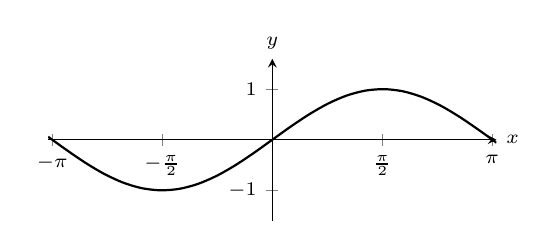
\begin{tikzpicture}
 \begin{axis}[width=.6\textwidth,height=.3\textwidth,
   tick label style={font=\scriptsize},axis y line=middle,axis x line=middle,
   ymin=-1.6,ymax=1.6,xmin=-3.2,xmax=3.2,xtick={-3.14,-1.57,1.57,3.14},
   xticklabels={$-\pi$,$-\frac\pi2$,$\frac\pi2$,$\pi$},name=myplot]
  \addplot [{\colorone},smooth,thick,domain=-3.2:3.2] (x,{sin(deg(x))});
 \end{axis}
 \node [right] at (myplot.right of origin) {\scriptsize $x$};
 \node [above] at (myplot.above origin) {\scriptsize $y$};
\end{tikzpicture}
\end{center}

In order to find an appropriate restriction of the domain of $f$, we look for consecutive critical points where $f$ takes on its minimum and maximum values. In this case, we use the interval $[-\pi/2,\pi/2]$. The graph of $f$ over this interval is sketched below.

\begin{center}
\begin{tikzpicture}
 \begin{axis}[width=.6\textwidth,height=.45\textwidth,
   tick label style={font=\scriptsize},axis y line=middle,axis x line=middle,
   ymin=-1.5,ymax=1.5,xmin=-2,xmax=2,xtick={-1.57,1.57},
   xticklabels={$-\frac\pi2$,$\frac\pi2$},name=myplot]
  \addplot [{\colorone},smooth,thick,domain=-1.57:1.57] (x,{sin(deg(x))});
 \end{axis}
 \node [right] at (myplot.right of origin) {\scriptsize $x$};
 \node [above] at (myplot.above origin) {\scriptsize $y$};
\end{tikzpicture}
\end{center}

We define the inverse of $f$ on this restricted range by $y=\arcsin x$ if and only if $\sin y=x$ and $-\pi/2\leq y\leq \pi/2$. The graph is a reflection of the graph of $g$ across the line $y=x$:

\begin{center}
\begin{tikzpicture}
 \begin{axis}[width=.45\textwidth,height=.6\textwidth,
   tick label style={font=\scriptsize},axis y line=middle,axis x line=middle,
   ymin=-2,ymax=2,xmin=-1.5,xmax=1.5,ytick={-1.57,1.57},
   yticklabels={$-\frac\pi2$,$\frac\pi2$},name=myplot]
  \addplot [{\colorone},smooth,thick,domain=-1.57:1.57] ({sin(deg(x))},x);
 \end{axis}
 \node [right] at (myplot.right of origin) {\scriptsize $x$};
 \node [above] at (myplot.above origin) {\scriptsize $y$};
\end{tikzpicture}
\end{center}

\subsection*{The inverse tangent function}

Next we consider the function $f(x)=\tan x$, which is also not one-to-one. A piece of the graph of $f$ is given below.

\begin{center}
\begin{tikzpicture}
 \begin{axis}[width=\textwidth,height=.6\textwidth,
   tick label style={font=\scriptsize},axis y line=middle,axis x line=middle,
   ymin=-3,ymax=3,xmin=-5,xmax=5,xtick={-4.71,-3.14,-1.57,1.57,3.14,4.71},
   xticklabels={$-\frac{3\pi}2$,$-\pi$,$\frac\pi2$,$\frac\pi2$,$\pi$,$\frac{3\pi}2$},
   name=myplot]
  \addplot [{\colorone},smooth,thick,domain=-1.5:1.5] (x,{tan(deg(x))});
  \addplot [{\colorone},smooth,thick,domain=-1.5:1.5] (x+3.14,{tan(deg(x))});
  \addplot [{\colorone},smooth,thick,domain=-1.5:1.5] (x-3.14,{tan(deg(x))});
 \end{axis}
 \node [right] at (myplot.right of origin) {\scriptsize $x$};
 \node [above] at (myplot.above origin) {\scriptsize $y$};
\end{tikzpicture}
\end{center}

In order to find an interval on which the function is one-to-one and on which the function takes on all values in the range, we use an interval between consecutive vertical asymptotes. Traditionally, the interval $(-\pi/2,\pi/2)$ is chosen. Note that we choose the open interval in this case because the function $f$ is not defined at the endpoints. So we define $y=\arctan x$ if and only if $\tan y=x$ and $-\pi/2< y<\pi/2$. The graph of $y=\arctan x$ is shown below. Note that the vertical asymptotes of the original function are reflected to become horizontal asymptotes of the inverse function.

\begin{center}
\begin{tikzpicture}
 \begin{axis}[width=\textwidth,height=.5\textwidth,name=myplot,
   tick label style={font=\scriptsize},axis y line=middle,axis x line=middle,
   ymin=-2,ymax=2,xmin=-4,xmax=4,ytick={-1.57,1.57},
   yticklabels={$\frac\pi2$,$\frac\pi2$}]
  \addplot [{\colorone},smooth,thick,domain=-1.5:1.5] ({tan(deg(x))},x);
 \end{axis}
 \node [right] at (myplot.right of origin) {\scriptsize $x$};
 \node [above] at (myplot.above origin) {\scriptsize $y$};
\end{tikzpicture}
\end{center}

\printexercises{exercises/07_07_exercises}

% todo add to 07_07_exset_02: cos(x)
